%%%%%%%%%%%%%%%%%%%%%%%%%%%%%%%%%%%%%%%%%%%%%%%%%%%%%%%%%%%%%%%
%% OXFORD THESIS TEMPLATE

% Use this template to produce a standard thesis that meets the Oxford University requirements for DPhil submission
%
% Originally by Keith A. Gillow (gillow@maths.ox.ac.uk), 1997
% Modified by Sam Evans (sam@samuelevansresearch.org), 2007
% Modified by John McManigle (john@oxfordechoes.com), 2015
% Modified by Ulrik Lyngs (ulrik.lyngs@cs.ox.ac.uk), 2018-, for use with R Markdown
%
% Ulrik Lyngs, 25 Nov 2018: Following John McManigle, broad permissions are granted to use, modify, and distribute this software
% as specified in the MIT License included in this distribution's LICENSE file.
%
% John commented this file extensively, so read through to see how to use the various options.  Remember that in LaTeX,
% any line starting with a % is NOT executed.

%%%%% PAGE LAYOUT
% The most common choices should be below.  You can also do other things, like replace "a4paper" with "letterpaper", etc.

% 'twoside' formats for two-sided binding (ie left and right pages have mirror margins; blank pages inserted where needed):
%\documentclass[a4paper,twoside]{templates/ociamthesis}
% Specifying nothing formats for one-sided binding (ie left margin > right margin; no extra blank pages):
%\documentclass[a4paper]{ociamthesis}
% 'nobind' formats for PDF output (ie equal margins, no extra blank pages):
%\documentclass[a4paper,nobind]{templates/ociamthesis}

% As you can see from the line below, oxforddown uses the a4paper size, 
% and passes in the binding option from the YAML header in index.Rmd:
\documentclass[a4paper, nobind]{templates/ociamthesis}


%%%%% ADDING LATEX PACKAGES
% add hyperref package with options from YAML %
\usepackage[pdfpagelabels]{hyperref}
% handle long urls
\usepackage{xurl}
% change the default coloring of links to something sensible
\usepackage{xcolor}

\definecolor{mylinkcolor}{RGB}{0,0,139}
\definecolor{myurlcolor}{RGB}{0,0,139}
\definecolor{mycitecolor}{RGB}{0,33,71}

\hypersetup{
  hidelinks,
  colorlinks,
  linktocpage=true,
  linkcolor=mylinkcolor,
  urlcolor=myurlcolor,
  citecolor=mycitecolor
}


% add float package to allow manual control of figure positioning %
\usepackage{float}

% enable strikethrough
\usepackage[normalem]{ulem}

% use soul package for correction highlighting
\usepackage{color, soulutf8}
\definecolor{correctioncolor}{HTML}{CCCCFF}
\sethlcolor{correctioncolor}
\newcommand{\ctext}[3][RGB]{%
  \begingroup
  \definecolor{hlcolor}{#1}{#2}\sethlcolor{hlcolor}%
  \hl{#3}%
  \endgroup
}
% stop soul from freaking out when it sees citation commands
\soulregister\ref7
\soulregister\cite7
\soulregister\citet7
\soulregister\autocite7
\soulregister\textcite7
\soulregister\pageref7

%%%%% FIXING / ADDING THINGS THAT'S SPECIAL TO R MARKDOWN'S USE OF LATEX TEMPLATES
% pandoc puts lists in 'tightlist' command when no space between bullet points in Rmd file,
% so we add this command to the template
\providecommand{\tightlist}{%
  \setlength{\itemsep}{0pt}\setlength{\parskip}{0pt}}
 
% allow us to include code blocks in shaded environments

% User-included things with header_includes or in_header will appear here
% kableExtra packages will appear here if you use library(kableExtra)
\usepackage{booktabs}
\usepackage{longtable}
\usepackage{array}
\usepackage{multirow}
\usepackage{wrapfig}
\usepackage{float}
\usepackage{colortbl}
\usepackage{pdflscape}
\usepackage{tabu}
\usepackage{threeparttable}
\usepackage{threeparttablex}
\usepackage[normalem]{ulem}
\usepackage{makecell}
\usepackage{xcolor}


%UL set section header spacing
\usepackage{titlesec}
% 
\titlespacing\subsubsection{0pt}{24pt plus 4pt minus 2pt}{0pt plus 2pt minus 2pt}


%UL set whitespace around verbatim environments
\usepackage{etoolbox}
\makeatletter
\preto{\@verbatim}{\topsep=0pt \partopsep=0pt }
\makeatother


%%%%%%% PAGE HEADERS AND FOOTERS %%%%%%%%%
\usepackage{fancyhdr}
\setlength{\headheight}{15pt}
\fancyhf{} % clear the header and footers
\pagestyle{fancy}
\renewcommand{\chaptermark}[1]{\markboth{\thechapter. #1}{\thechapter. #1}}
\renewcommand{\sectionmark}[1]{\markright{\thesection. #1}} 
\renewcommand{\headrulewidth}{0pt}

\fancyhead[LO]{\emph{\leftmark}} 
\fancyhead[RE]{\emph{\rightmark}} 




% UL page number position 
\fancyfoot[C]{\emph{\thepage}} %regular pages
\fancypagestyle{plain}{\fancyhf{}\fancyfoot[C]{\emph{\thepage}}} %chapter pages




%%%%% SELECT YOUR DRAFT OPTIONS
% This adds a "DRAFT" footer to every normal page.  (The first page of each chapter is not a "normal" page.)

% IP feb 2021: option to include line numbers in PDF

% for line wrapping in code blocks
\usepackage{fancyvrb}
\usepackage{fvextra}
\DefineVerbatimEnvironment{Highlighting}{Verbatim}{breaklines=true, breakanywhere=true, commandchars=\\\{\}}

% This highlights (in blue) corrections marked with (for words) \mccorrect{blah} or (for whole
% paragraphs) \begin{mccorrection} . . . \end{mccorrection}.  This can be useful for sending a PDF of
% your corrected thesis to your examiners for review.  Turn it off, and the blue disappears.
\correctionstrue


%%%%% BIBLIOGRAPHY SETUP
% Note that your bibliography will require some tweaking depending on your department, preferred format, etc.
% If you've not used LaTeX before, I recommend just using pandoc for citations -- this is what's used unless you specific e.g. "citation_package: natbib" in index.Rmd
% If you're already a LaTeX pro and are used to natbib or something, modify as necessary.

% this allows the latex template to handle pandoc citations
\newlength{\cslhangindent}
\setlength{\cslhangindent}{1.5em}
\newlength{\csllabelwidth}
\setlength{\csllabelwidth}{3em}
\newlength{\cslentryspacingunit} % times entry-spacing
\setlength{\cslentryspacingunit}{\parskip}
\newenvironment{CSLReferences}[2] % #1 hanging-ident, #2 entry spacing
 {% don't indent paragraphs
  \setlength{\parindent}{0pt}
  % turn on hanging indent if param 1 is 1
  \ifodd #1
  \let\oldpar\par
  \def\par{\hangindent=\cslhangindent\oldpar}
  \fi
  % set entry spacing
  \setlength{\parskip}{1mm}
  \setlength{\baselineskip}{6mm}
 }%
 {}
\usepackage{calc}
\newcommand{\CSLBlock}[1]{#1\hfill\break}
\newcommand{\CSLLeftMargin}[1]{\parbox[t]{\csllabelwidth}{#1}}
\newcommand{\CSLRightInline}[1]{\parbox[t]{\linewidth - \csllabelwidth}{#1}\break}
\newcommand{\CSLIndent}[1]{\hspace{\cslhangindent}#1}




% Uncomment this if you want equation numbers per section (2.3.12), instead of per chapter (2.18):
%\numberwithin{equation}{subsection}


%%%%% THESIS / TITLE PAGE INFORMATION
% Everybody needs to complete the following:
\title{\texttt{Feasibility\ and\ Acceptance\ of\ chatbots\ embedded\ in\ healthcare\ curricula}:}
\author{Matthew Pears- with CEPEH Team James Henderson, Natalia Stathakarou, Klas Karlgren, ,Panagiotis D Bamidis, Iraklis Tsoupouroglou, Eirini Schiza, Constantinos S Pattichis, and Stathis Th Konstantinidis}
\college{CEPEH report 2023}

% Master's candidates who require the alternate title page (with candidate number and word count)
% must also un-comment and complete the following three lines:

% Uncomment the following line if your degree also includes exams (eg most masters):
%\renewcommand{\submittedtext}{Submitted in partial completion of the}
% Your full degree name.  (But remember that DPhils aren't "in" anything.  They're just DPhils.)
\degree{December}

% Term and year of submission, or date if your board requires (eg most masters)
\degreedate{2023}


%%%%% YOUR OWN PERSONAL MACROS
% This is a good place to dump your own LaTeX macros as they come up.

% To make text superscripts shortcuts
\renewcommand{\th}{\textsuperscript{th}} % ex: I won 4\th place
\newcommand{\nd}{\textsuperscript{nd}}
\renewcommand{\st}{\textsuperscript{st}}
\newcommand{\rd}{\textsuperscript{rd}}

%%%%% THE ACTUAL DOCUMENT STARTS HERE
\begin{document}

%%%%% CHOOSE YOUR LINE SPACING HERE
% This is the official option.  Use it for your submission copy and library copy:
\setlength{\textbaselineskip}{22pt plus2pt}
% This is closer spacing (about 1.5-spaced) that you might prefer for your personal copies:
%\setlength{\textbaselineskip}{18pt plus2pt minus1pt}

% You can set the spacing here for the roman-numbered pages (acknowledgements, table of contents, etc.)
\setlength{\frontmatterbaselineskip}{17pt plus1pt minus1pt}

% UL: You can set the line and paragraph spacing here for the separate abstract page to be handed in to Examination schools
\setlength{\abstractseparatelineskip}{13pt plus1pt minus1pt}
\setlength{\abstractseparateparskip}{0pt plus 1pt}

% UL: You can set the general paragraph spacing here - I've set it to 2pt (was 0) so
% it's less claustrophobic
\setlength{\parskip}{2pt plus 1pt}

%
% Customise title page
%
\def\crest{{
\includegraphics[width=5cm]{templates/download.png}}}
\renewcommand{\university}{--}
\renewcommand{\submittedtext}{}
\renewcommand{\thesistitlesize}{\fontsize{22pt}{28pt}\selectfont}
\renewcommand{\gapbeforecrest}{25mm}
\renewcommand{\gapaftercrest}{25mm
}


% Leave this line alone; it gets things started for the real document.
\setlength{\baselineskip}{\textbaselineskip}


%%%%% CHOOSE YOUR SECTION NUMBERING DEPTH HERE
% You have two choices.  First, how far down are sections numbered?  (Below that, they're named but
% don't get numbers.)  Second, what level of section appears in the table of contents?  These don't have
% to match: you can have numbered sections that don't show up in the ToC, or unnumbered sections that
% do.  Throughout, 0 = chapter; 1 = section; 2 = subsection; 3 = subsubsection, 4 = paragraph...

% The level that gets a number:
\setcounter{secnumdepth}{2}
% The level that shows up in the ToC:
\setcounter{tocdepth}{1}


%%%%% ABSTRACT SEPARATE
% This is used to create the separate, one-page abstract that you are required to hand into the Exam
% Schools.  You can comment it out to generate a PDF for printing or whatnot.

% JEM: Pages are roman numbered from here, though page numbers are invisible until ToC.  This is in
% keeping with most typesetting conventions.
\begin{romanpages}

% Title page is created here
\maketitle

%%%%% DEDICATION
\begin{dedication}
  see cepeh.eu for more information
\end{dedication}

%%%%% ACKNOWLEDGEMENTS


\begin{acknowledgements}
 	This work is supported by the ERASMUS+ Strategic Partnership in Higher Education ``Chatbot Enhance Personalise European Healthcare Curricula (CEPEH)'' (www.cepeh.eu) (2019-1-UK01- KA203-062091) project of the European Union.

 Thanks to Mohammed Roshan for data processing.

 \begin{flushright}
 CEPEH Team \\
 \end{flushright}
\end{acknowledgements}



%%%%% ABSTRACT


\renewcommand{\abstracttitle}{Abstract}
\begin{abstract}
	This document details the evaluation of each resource in terms of the feasibility and acceptance from the end-users. There was evidence of identifying the feasibility of such resources into formal training and studies exist on the acceptance of such resources, with promising results. However, all these studies defined the need for further research in the area until the use of chatbots in healthcare education became common. Furthermore, the creation process of CEPEH resources was significantly different and had improvements to current methods, due to the co-creation process, and use of low cost but effective technology.
\end{abstract}



%%%%% MINI TABLES
% This lays the groundwork for per-chapter, mini tables of contents.  Comment the following line
% (and remove \minitoc from the chapter files) if you don't want this.  Un-comment either of the
% next two lines if you want a per-chapter list of figures or tables.
\dominitoc % include a mini table of contents

% This aligns the bottom of the text of each page.  It generally makes things look better.
\flushbottom

% This is where the whole-document ToC appears:
\tableofcontents

\listoffigures
	\mtcaddchapter
  	% \mtcaddchapter is needed when adding a non-chapter (but chapter-like) entity to avoid confusing minitoc

% Uncomment to generate a list of tables:
\listoftables
  \mtcaddchapter
%%%%% LIST OF ABBREVIATIONS
% This example includes a list of abbreviations.  Look at text/abbreviations.tex to see how that file is
% formatted.  The template can handle any kind of list though, so this might be a good place for a
% glossary, etc.
% First parameter can be changed eg to "Glossary" or something.
% Second parameter is the max length of bold terms.
\begin{mclistof}{List of Abbreviations}{3.2cm}

\item[CEPEH]

Chatbot Enhance Personalised European Healthcare curricula

\item[HELM]

Health E-Learning and Media team

\item[RLO]

Reusable Learning Object

\item[ASPIRE]

Aims Storyboarding Production Implementation Release Evaluation

\item[NLP]

Natural Language Processing

\item[NLU]

Natural Language Understanding

\item[A.I]

Artificial Intelligence

\item[TAM]

Technology Acceptance Model

\item[SUS]

System Usability Scale

\item[CUQ]

Chatbot Usability Questionnaire

\item[HIG]

HELM is Great

\end{mclistof} 


% The Roman pages, like the Roman Empire, must come to its inevitable close.
\end{romanpages}

%%%%% CHAPTERS
% Add or remove any chapters you'd like here, by file name (excluding '.tex'):
\flushbottom

% all your chapters and appendices will appear here
\hypertarget{introduction}{%
\chapter*{Introduction}\label{introduction}}
\addcontentsline{toc}{chapter}{Introduction}

\adjustmtc
\markboth{Introduction}{}

Personalised Healthcare Education is needed to meet growing demand and quality maintenance.
There is a growing evidence around chatbots, namely machine conversation systems- these programs have the potential to change the way students learn and search for information.

Chatbots can quiz existing knowledge, enable higher student engagement with a learning task, or support higher-order cognitive activities.
In large-scale learning scenarios with a hight student-to-lecturer ratio, chatbots can help tackle the issue of individualized student support and facilitate personalised learning.
However, limited examples of chatbots in European Healthcare Curricula have been utilised to combine both the continuum of cognitive processes presented in Bloom's taxonomy, with the idea that some repetitive tasks can be done with a chatbot- to provide greater access or to scale faculty time.

Thus, CEPEH strategic partnership has co-created open access chatbots utilising artificial intelligence, promoting innovative practices in digital era, by supporting current curricula and fostering open education.

CEPEH Erasmus+ strategic partnership aimed to co-design and implement new pedagogical approaches and, in particular, chatbots for European medical and nursing schools.
CEPEH used use participatory design to engage stakeholders (students, healthcare workforce staff, lecturers, clinicians, etc.) in order to co-design effective chatbots and release them as open access resources.
Through CEPEH, effective use of digital technologies and open education were be incorporated into healthcare curricula.
This enabled students to increase their health and medical related skills through flexible learning.

CEPEH expected that students adopted this new digital pedagogy and improve their skills and competences through flexible personalised learning, while the teaching staff enhanced their e-learning tool co-creation competences and make use of co-design best practices and recommendations for use.
It is also expected increased cooperation between the partners.
Thus, in the long term, CEPEH expects to influence the development of medical and nursing curricula with this digital innovation, foster the quality of the future healthcare workforce and further improve international competitiveness of the partners' healthcare curricula.
This document details the evaluation of the resources created by the CEPEH team.

The evaluation specifically explored the feasibility and acceptance from the end-users.
These end-users are learners in European healthcare higher education institutions.

There was firstly evidence for the need to identify the feasibility of chatbots and similar resources into formal education and training, with a further need to improve access to these types of learning resources.
Of course, studies exist on the acceptance of chatbots, virtual patients, and many other healthcare applications, with promising results.
However, through various limitations, we believed there was further research to be completed to accelerate the design, development, implementation, and evaluation processes.
These have financial, stakeholder, time, and efficacy benefits.
The creation process of CEPEH resources was significantly different to most in the literature, and this report highlights the approach of the CEPEH team towards enhancing personalised healthcare education can be achieved.

\hypertarget{sec-background}{%
\section*{Background}\label{sec-background}}
\addcontentsline{toc}{section}{Background}

The working practices of CEPEH are aimed at maximizing efficacy of these chatbots as learning resources, and provided a sense of shared development and ownership from all stakeholders.
The process normally begins with workshops in which the project is scoped and team building occurs.
The CEPEH workshops involve the widest possible team of stakeholders including tutors, students, healthcare workers, learning technologists, health service users and carers- depending on the materials being created.

For readers who are interested in using these high quality digital resources please access them for free at CEPEH.EU

The next section will now present the evaluation of all CEPEH chatbot resources.

\hypertarget{method}{%
\chapter{Method}\label{method}}

\minitoc 

\hypertarget{participants}{%
\section{Participants}\label{participants}}

This dataset had 14 males and 28 females therefore a total of 42 participants.
It was a repeated measure design whereby each participant used the 4 chatbots developed by the CEPEH team.
Therefore, there are 42 points of data in the condition before testing, and 126 data points after testing the chatbots- for a total of 168 row of data, 5 per participant.
There were 78 questions asked in total, therefore the full dataset has over 4000 cells recorded.

There were 22 females and 7 males from Greece.
There were 3 females and 4 males from Cyprus.
There were 2 females and 2 males from Sweden,
and there were 2 participants from the United Kingdom (see(\ref{fig:location1}).

\begin{figure}
\centering
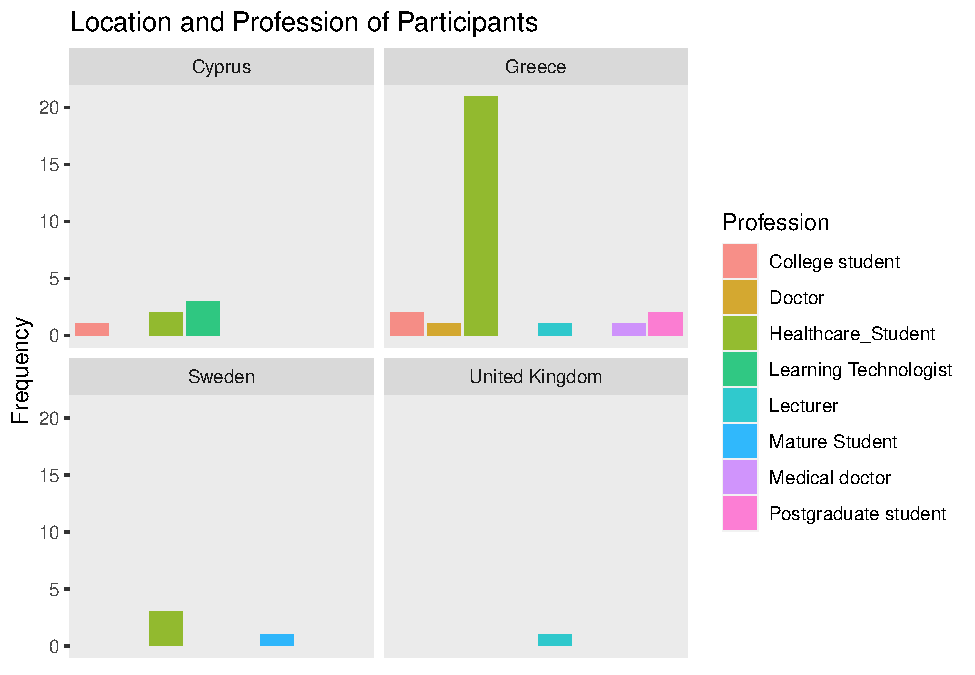
\includegraphics{_main_files/figure-latex/location1-1.pdf}
\caption{\label{fig:location1}Location and Profession of Participants}
\end{figure}

The majority 36 participants, were student, with 3 being learning technologists, 2 were lecturers, and 1 was a doctor.
Although there could be a difference in these groups, the design was within- groups therefore each participants pre-usage metrics were the comparative control data, and participant differences did not affect the evaluation.

\hypertarget{procedure}{%
\section{Procedure}\label{procedure}}

For each resource created by the Partners, the same experimental methodology was followed.
For each resource created by partners, students performed a study within an online or face to face workshop or course.
Student participants joined from Greece, Cyprus, Sweden, and the United Kingdom.
A repeated measures design was used as the same group measures were taken before and after usage of the chatbots.
They were recruited via staff members in the CEPEH group.

Participants were asked prior to the study if they agree to participate, providing them with a PIS form.
Participants had the opportunity to discuss with the research team prior to the study and before consent is given.
Then, participants used the chatbot resources independently and technical support was provided.
Finally, post-intervention measures were recorded.

Some of the participants were invited to participate in Focus Group Discussions (FGD), and each FGD lasted between 15 to 25 minutes, with 5-10 participants.
Participants were asked if they would like to be informed of the findings of the study.

\hypertarget{design}{%
\section{Design}\label{design}}

The data captured from the participants were their initials and numerical day of birth, used as anonymous identifier for pre-post analysis.
Their institution was captured (Aristotle University of Thessaloniki, CYENS Centre of Excellent, Karolinska Institute, and The University of Nottingham), and Sex (Male/Female/Other).

Before any interaction with the learning resources, various perceptions of chatbot such as confidence and easy of use, usefulness, Influence from others, and current learning resources (videos, textbooks, Google, friends etc), were captured.
Descriptive data was produced alongside repeated measures t-tests.
Repeated measures t-tests were the appropriate test to use as this explores differences between groups, there were no covariates and we did not have several dependant variables.
There was one Independent factor being Chatbot use having 2 levels (pre/post).
There were 3 chatbots therefore there was option for ANOVA to determine where differences lie if statistical differences were found however this was not wholly appropriate for the data type and not necessary for pre-post comparison.

\#\# Materials and Measures

The measures used fit within a newly developed Chatbot Evaluation Framework- which takes the best measures of 5 previous frameworks.
Denecke and Warren \hspace{0pt}{[}2{]}\hspace{0pt} derived several quality dimensions and attributes from previous chatbot literature.
They formed six perspectives from their review of articles and mobile health applications.

These six perspectives were: 1) Task-oriented, 2) Artificial intelligence, 3) System quality perspective, 4) Linguistic perspective, 5) UX Perspective, 6) Healthcare quality perspective.

To capture these perspectives, we used several validated materials that can distinguish these elements of the CEPEH chatbots.

\hypertarget{chatbot-usability-questionnaire-cuq}{%
\subsection{Chatbot Usability Questionnaire (CUQ)}\label{chatbot-usability-questionnaire-cuq}}

The Chatbot Usability Questionnaire (CUQ) \hspace{0pt}{[}4{]}\hspace{0pt} is a new questionnaire specifically designed for measuring the usability of chatbots by an interdisciplinary team from the Ulster University.
CUQ can be used alongside the prevalent System Usability Scale Score (SUS) \hspace{0pt}{[}5{]}\hspace{0pt}.
Multiple metrics are more appropriate when measuring usability of chatbots \hspace{0pt}{[}6{]}\hspace{0pt} therefore a combination of two scores can provide an all-inclusive overview.

\hypertarget{utaut2-unified-theory-of-acceptance-and-use-of-technology}{%
\subsection{UTAUT2 (Unified Theory of Acceptance and Use of Technology)}\label{utaut2-unified-theory-of-acceptance-and-use-of-technology}}

The underpinning theory of the UTAUT2 is that there are four key constructs to the intentions of using technology based resources: 1) performance expectancy, 2) effort expectancy, 3) social influence, and 4) enabling conditions.

The TAM and the UTAUT2 have cross over in measuring technology acceptance, however the UTAUT2 has more applied probing questions.
Few studies exist that use technology acceptance theories for the intention to use products that explicitly incorporate AI.
A recent extension of the UTAUT2 model added five (health, convenience comfort, sustainability, safety, security, and personal innovativeness) additional influencing factors to accommodate for AI {[}7{]}.
This can be used for products in either health, household use, or mobility and can help to explain behavioural intention and use behaviour of chatbots.

\hypertarget{system-usability-scale}{%
\subsection{System Usability Scale}\label{system-usability-scale}}

The System Usability Scale (SUS) was used {[}10{]} and is a widely used and adopted usability questionnaire.
It is popular due to its unbiased and agnostic properties, a non proprietary, and a quick scale of 10 questions. However, as there are the CUQ and parts of the UTAUT2 we have selected only 2 questions which do not cross-over with the other measures. These are improtant statements however and good indicators of usability when assessed with the other results.

\hypertarget{computer-self-efficacy-scale-tool}{%
\subsection{Computer Self-Efficacy Scale Tool}\label{computer-self-efficacy-scale-tool}}

The 10 question CSEST is based on the 32-item questionnaire by Murphy, Coover, and Owen (1989). It can be adapted for any technology and we have selected only a few pertinent questions. Participants are asked to think about using the CEPEH chatbots and answer that they would use the chatbots if I had never used a product like it before; If they could call someone for help if I got stuck, or if someone showed them how to do it first, and other similar usage questions.

\hypertarget{technology-acceptance-model-tam}{%
\subsection{Technology Acceptance Model (TAM)}\label{technology-acceptance-model-tam}}

The Technology Acceptance Model (TAM) {[}1{]} was specifically developed with the primary aim of identifying the determinants involved in computer acceptance in general; secondly, to examine a variety of information technology usage behaviours; and thirdly, to provide a parsimonious theoretical explanatory model.

TAM suggests that attitude would be a direct predictor of the intention to use technology, which in turn would predict the actual usage of the technology.
The only modification to the nine sub-scales of the questionnaire consists of applying the items to the context of chatbots.
All the items, except those measuring attitudes, utilize a seven-point Likert scale ranging from ``strongly agree'' to ``strongly disagree'' with a middle neutral point {[}2{]}.

The nine sub-scales of the questionnaire:

• Ease of use of chatbots
• Perceived usefulness of chatbots
• Intention of use.
• Attitude toward usage of chatbots.
• Perception of personal efficacy to use a chatbot resource.
• Perception of external control toward chatbots.
• Anxiety toward chatbot use.
• Intrinsic motivation to use chatbot resources.
• Perceived costs of chatbots.

\hypertarget{qualitative-measure--focus-group-discussions}{%
\subsection{Qualitative Measure- Focus Group Discussions}\label{qualitative-measure--focus-group-discussions}}

Focus groups are a pervasive means of market research and provides credible acceptance evaluators regarding the penetration that a product or service will have on a target demographic.Focus groups are a form of qualitative research consisting of interviews or structured discussions, in which a group of people are asked about their perceptions, opinions, beliefs, and attitudes towards a product, service, concept, advertisement, idea, or packaging.

Questions are asked in an interactive group setting where participants are free to talk with other group members.During this process, the researcher either takes notes or records the vital points he or she is getting from the group.
Researchers select members of the focus group carefully for effective and authoritative responses.Relevant stakeholders, then, can use the information collected through focus groups to receive insights on a specific product, issue, or topic focus {[}7{]}.

A series of short focus group sessions identified the feasibility of CEPEH resources for formal curricular integration.These sessions, spanning no more than 1-1.5 hours and consisting of no more than 5-7 persons each explored all axes of curricular integration such as accessibility in the classroom, use case scenarios, technology requirements for curricular integration etc.These axes were formalized by the research team, in each evaluation site, to consider the curricular details of each institution.

\includegraphics[width=5.76in]{untitled-1}

Figure 1: Flow diagram of the recruitment process

\hypertarget{rmd-basics}{%
\chapter{Results}\label{rmd-basics}}

\minitoc 

\noindent

\hypertarget{participants-characteristics}{%
\section{Participants' Characteristics}\label{participants-characteristics}}

When participants were asked the amount of time they have used a chatbot
in any form or subject, 23 stated they had never used a chatbot.
Further, 19/42 stated having used a chatbot at least once for between
0-4 hours of use in total. These are likely commercial/website- based
assistant chatbots however there are some medical/healthcare resources
known to be used in anatomy and/or patient interactions. One individual
had spent much longer time with usage- this was the mature student.

\begin{longtable}[]{@{}lr@{}}
\caption{Previous Chatbot Usage of Participants}\tabularnewline
\toprule()
Previous\_Chatbot\_Usage & n \\
\midrule()
\endfirsthead
\toprule()
Previous\_Chatbot\_Usage & n \\
\midrule()
\endhead
1-4 hours & 16 \\
10-19 hours & 1 \\
5-9 hours & 2 \\
Never & 23 \\
\bottomrule()
\end{longtable}

In short, approximately 50\% had never used a chatbot, and 45\% had used a
chatbot, at some period over the years, for a short period of time.

\begin{figure}
\centering
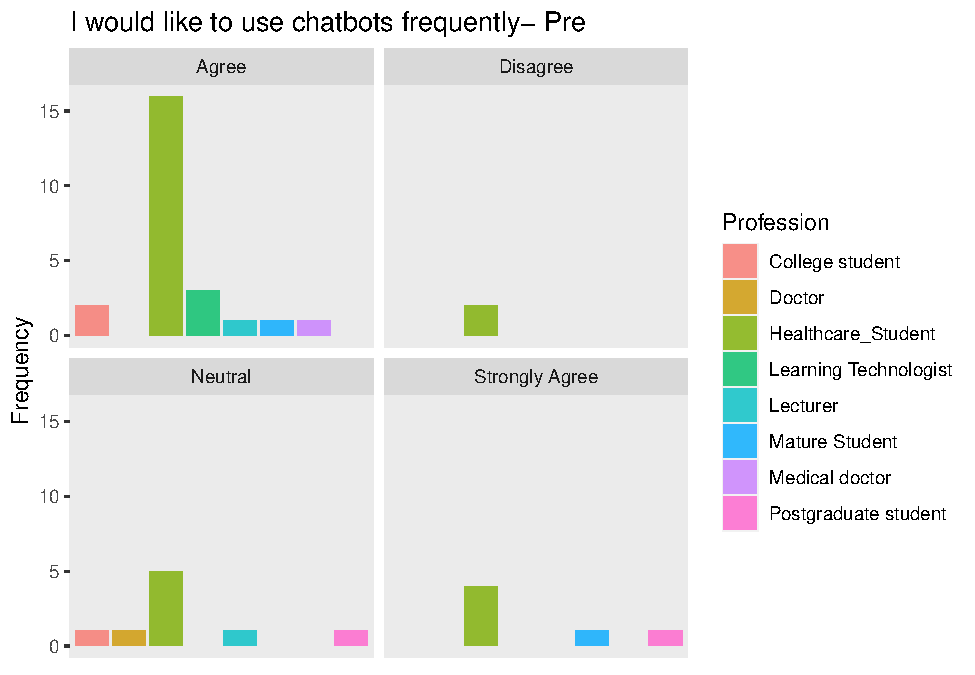
\includegraphics{_main_files/figure-latex/Boxplotsplits2-1.pdf}
\caption{\label{fig:Boxplotsplits2}Chatbot Usage History- Pre}
\end{figure}

Most learners use books or online books as resources. They may use
multiple sources however they were asked to note the primary source.
Only 6 stated their primary sources were \emph{Online videos/interactive
materials} which includes such tools as chatbots.

The first boxplot (\ref{fig:Boxplotsplits2}) shows learners perceptions
of easy of use of mobile app and other educational mobile resources

\begin{figure}
\centering
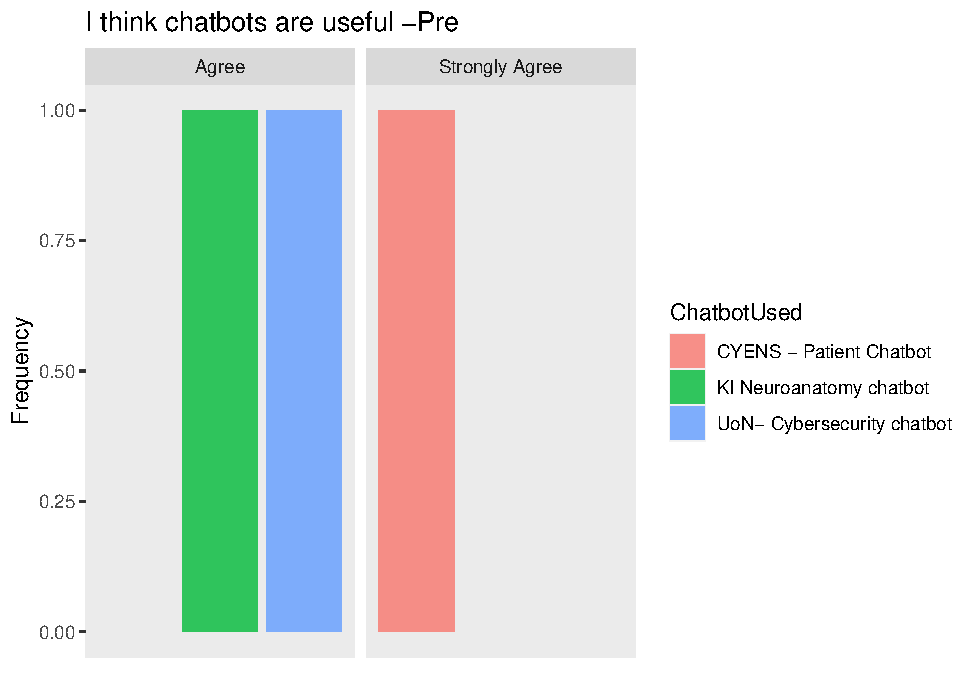
\includegraphics{_main_files/figure-latex/BoxplotUsefulPre-1.pdf}
\caption{\label{fig:BoxplotUsefulPre}Chatbots are Useful Opinion- Pre}
\end{figure}

(\ref{fig:BoxplotUsefulPre}) shows the opinions of all participants on
the usefulness of chatbots. Many had not had experience with them yet
had positive rating. This positive opinions of chatbots may be from
colleagues, friends, media, tutors, or other social information of the
benefits in healthcare education. Around 25\% were neutral or disagreed
that healthcare chatbots were useful.

\textbf{\emph{The participants then used the 4 chatbots, and completed the
post-usage survey after each chatbot. Results after use are as
followed:}}

\hypertarget{chatbot-usability-questionnaire-cuq-sec-chatbot-usability-questionnaire-cuq}{%
\section{Chatbot Usability Questionnaire (CUQ) \{\#sec-chatbot-usability-questionnaire-(cuq)\}}\label{chatbot-usability-questionnaire-cuq-sec-chatbot-usability-questionnaire-cuq}}

\hypertarget{cuq-calculation-tool}{%
\subsection{CUQ Calculation tool}\label{cuq-calculation-tool}}

The CUQ was developed by researchers at Ulster University,
\href{https://www.ulster.ac.uk/research/topic/computer-science/artificial-intelligence/projects/cuq}{Link}
and as the calculation can be complex, a dedicated calculation tool has
been created.

Please download the CEPEH CUQ calculation tool which has all of the data
entered, so you can see the CEPEH CUQ scoring

\href{CUQ-Calculation-Tool.xlsx}{Click here to download CUQ calc tool}

\href{cuq.png}{Click here to download CEPEH CUQ score result}

\begin{figure}

{\centering 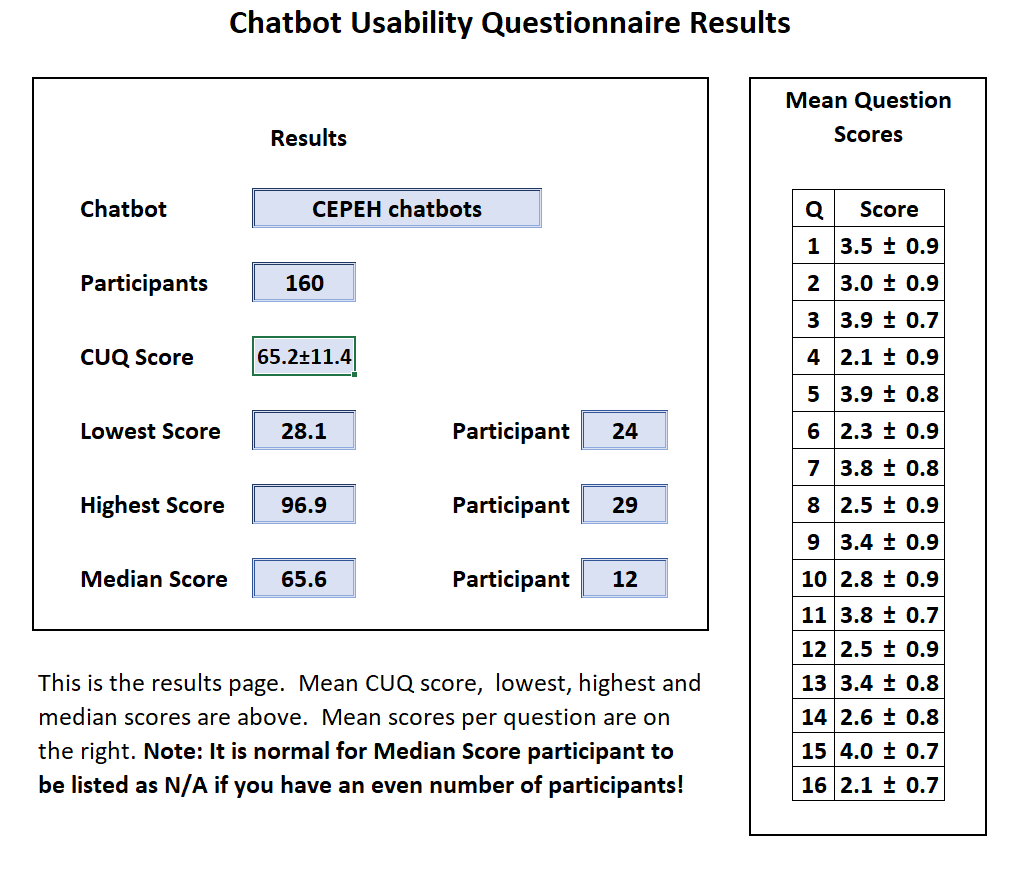
\includegraphics[width=0.75\linewidth]{cuq} 

}

\caption{CUQ CEPEH Score}\label{fig:cuqimage}
\end{figure}

Although the design and development was similar, each chatbot CUQ score
was calculated to understand how the topic content may affect usability:

The breakdown of the chatbots was:

\begin{itemize}
\tightlist
\item
  Aristotle University of Thessaloniki CUQ score = 63/100
\item
  CYENS Centre of Excellence CUQ score = 67/100
\item
  Karolinska Institute CUQ score = 63/100
\item
  University of Nottingham CUQ score = 68/100
\end{itemize}

The score for all 3 chatbots grouped was 65/100. See Discussion CUQ
section for interpretation

\begin{figure}

{\centering 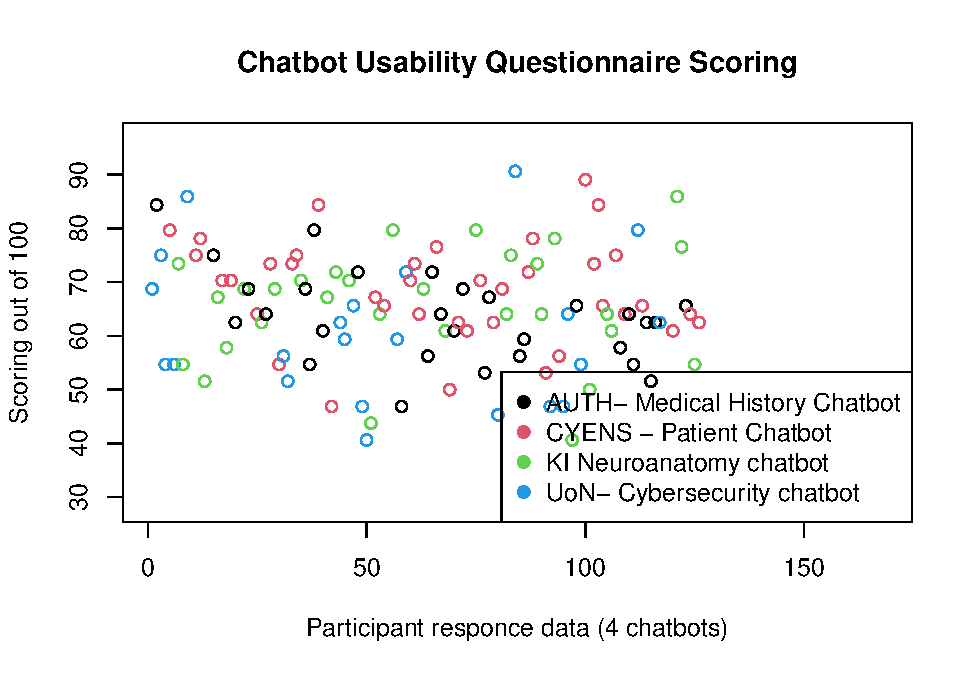
\includegraphics{_main_files/figure-latex/CUQscatterplot-1} 

}

\caption{CUQ Scatter Plot}\label{fig:CUQscatterplot}
\end{figure}

Figure (\ref{fig:CUQscatterplot}) shows the CUQ scores as a scatter
plot to highlight how there was a moderate distribution of results.
Further exploration is required to understand which elements are causing
this spread, and if it was due to problems within a small group of
learners.

\hypertarget{system-usability-scale-sus-scores-sec-system-usability-scale-sus-scores}{%
\section{System Usability Scale (SUS) Scores \{\#sec-system-usability-scale-(sus-scores)\}}\label{system-usability-scale-sus-scores-sec-system-usability-scale-sus-scores}}

\emph{Note= The amount of `agreement' is defined as the addition of `Agree'
and `Strongly agree' responses.}

The SUS score should consist of 10 items. However, some SUS questions
were improved upon by 1 or more CUQ questions, specifically to this
Chatbot study. The SUS results would be obscured by the CUQ scores,
expect 2 that did not have cross-over. The two questions were:

\begin{itemize}
\tightlist
\item
  I would like to use the CEPEH chatbot I tested, more frequently
  (SUS1)(post)
\item
  I felt confident using the CEPEH chatbot (SUS2)(post)
\end{itemize}

This meant the score of the SUS was not created, however the CUQ score
better represented the Learners' perceptions of the CEPEH chatbot in
terms of feasibility of use and acceptability in healthcare curricula.

\begin{longtable}[]{@{}lr@{}}
\toprule()
Confident & V1 \\
\midrule()
\endhead
Agree & 66 \\
Disagree & 15 \\
Neutral & 17 \\
Not Applicable & 3 \\
Strongly Agree & 23 \\
Strongly Disagree & 2 \\
\bottomrule()
\end{longtable}

This table above shows keep using chatbots

\begin{longtable}[]{@{}lr@{}}
\toprule()
Confidence using CEPEH Chatbot(s) & Responces \\
\midrule()
\endhead
Agree & 71 \\
Disagree & 11 \\
Neutral & 21 \\
Not Applicable & 4 \\
Strongly Agree & 19 \\
\bottomrule()
\end{longtable}

This table shows the distribution of agreement for participants for all
4 chatbots. The table shows 90/126 records that participants feel they
are confident in using the chatbots. However, 21/126 (16\%) were neutral
and 11/126 (8.5\%) disagreed and this was explored in the qualitative
analysis section.

\hypertarget{technology-acceptance-model}{%
\section{Technology Acceptance Model}\label{technology-acceptance-model}}

The TAM questions were analysed according to their subsets. The subsets
were Perceived Usefulness (PU) and Perceived Easy of Use (PEU)

The questions were: Perceived Usefulness (PU)

\begin{enumerate}
\def\labelenumi{\arabic{enumi}.}
\tightlist
\item
  Using CEPEH chatbots would enable me to accomplish tasks more
  quickly
\item
  Using CEPEH chatbots would increase performance
\item
  Using CEPEH chatbots would increase my productivity
\item
  I would find CEPEH chatbots useful on my course
\end{enumerate}

Perceived Easy of Use (PEU)

\begin{enumerate}
\def\labelenumi{\arabic{enumi}.}
\setcounter{enumi}{4}
\item
  Learning to use CEPEH chatbots would be easy to me
\item
  It would be easy for me to be skilful at using CEPEH chatbots
\item
  My interactions with CEPEH chatbots would be clear and
  understandable
\item
  I would find CEPEH chatbots easy to use
\end{enumerate}

Results:

The scores as a percentage of agreement, were calculated by averaging
the subsets and interpreted as:

Before using the CEPEH chatbots, there was 66\% (2.2/5) agreement for the
Perceived Usefulness of chatbots in healthcare education, and after 48\%
(2.6/5) agreed.

Before using the CEPEH chatbots, there was 64\% (2.3) agreement for
Perceived Ease of Use of chatbots in healthcare education, and after 51\%
(2.56) agreed.

The justification for this may be due to being early versions of
applications with limited functionality and functions which can be
difficult for user to experience the intended further range of features
and learning exercises.

\hypertarget{other-measeures}{%
\section{Other Measeures}\label{other-measeures}}

\hypertarget{knowledge-of-topics-after-use}{%
\subsection{Knowledge of Topics after Use}\label{knowledge-of-topics-after-use}}

\begin{figure}
\centering
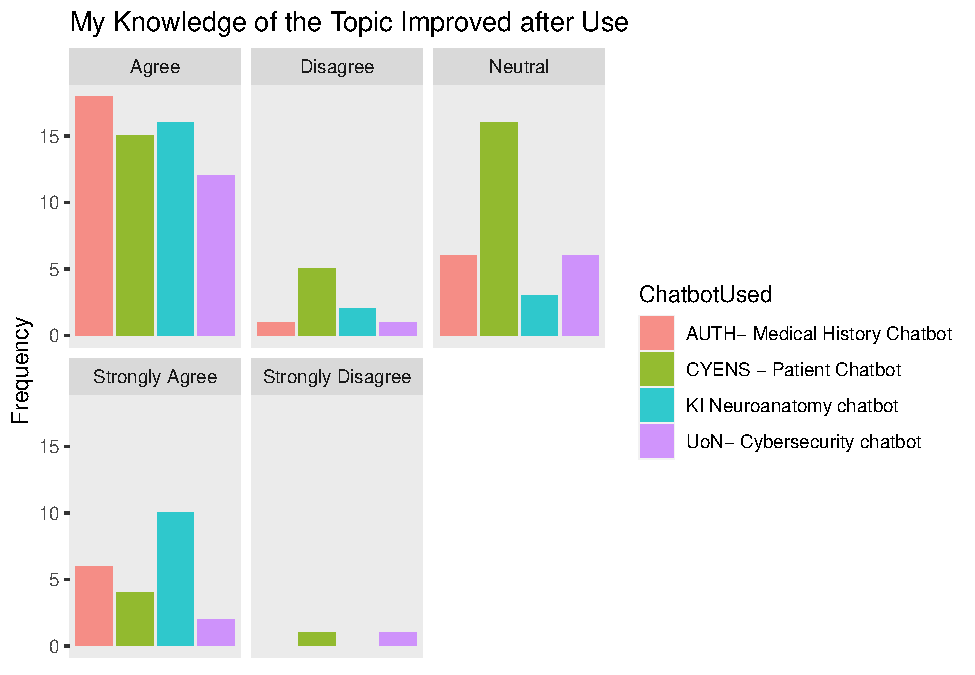
\includegraphics{_main_files/figure-latex/Boxplotsplits5-1.pdf}
\caption{\label{fig:Boxplotsplits5}Improvements in Knowledge}
\end{figure}

CYENS chatbot had around 10 more participants stating that they were
neutral on gaining knowledge of the topic

\hypertarget{trust-in-cepeh-chatbots-after-use}{%
\subsection{Trust in CEPEH chatbots after Use}\label{trust-in-cepeh-chatbots-after-use}}

\begin{figure}
\centering
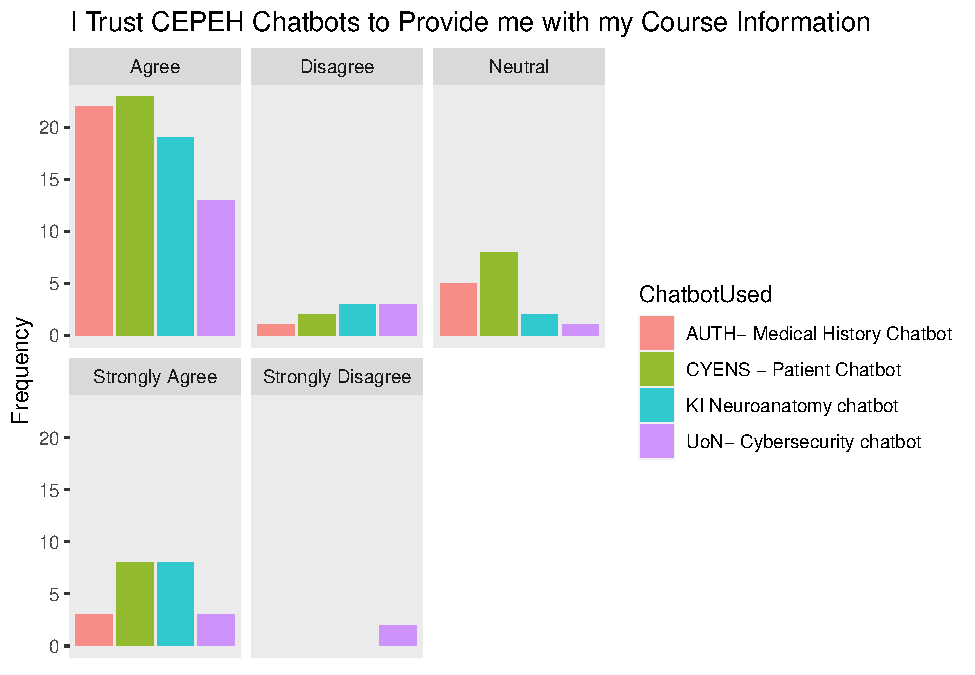
\includegraphics{_main_files/figure-latex/Boxplotsplits6-1.pdf}
\caption{\label{fig:Boxplotsplits6}Trust Chatbots POST use}
\end{figure}

The figure above, (\ref{fig:Boxplotsplits6}) shows the ratings by
participants of the CEPEH Chatbots to provide them with the necessary
course information. This is a integral element in learners' motivational
and educational choices to reuse the learning resources. As previously
described, the trust of the information is also a factor in these
responses.

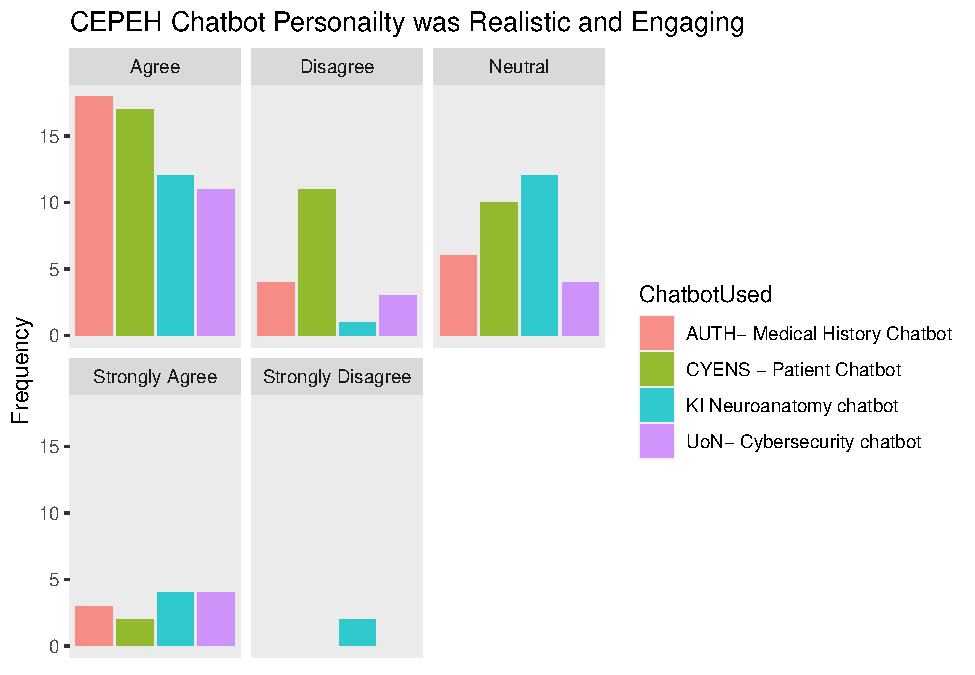
\includegraphics{_main_files/figure-latex/Boxplotsplits7-1.pdf}

There was mixed results for the chatbot used being realistic and
engaging. This question has two descriptive terms however based on the
other results we understand that the chatbots' NLP logic, or ability to
respond required improvement to be more `smooth' in replying. The
primary limitation was found in the `robotic' interactions(See Figure
10). This was investigated further in the `Text Mining' and `Sentiment
Analysis' sections.

\hypertarget{personailty-and-interactions}{%
\subsection{Personailty and Interactions}\label{personailty-and-interactions}}

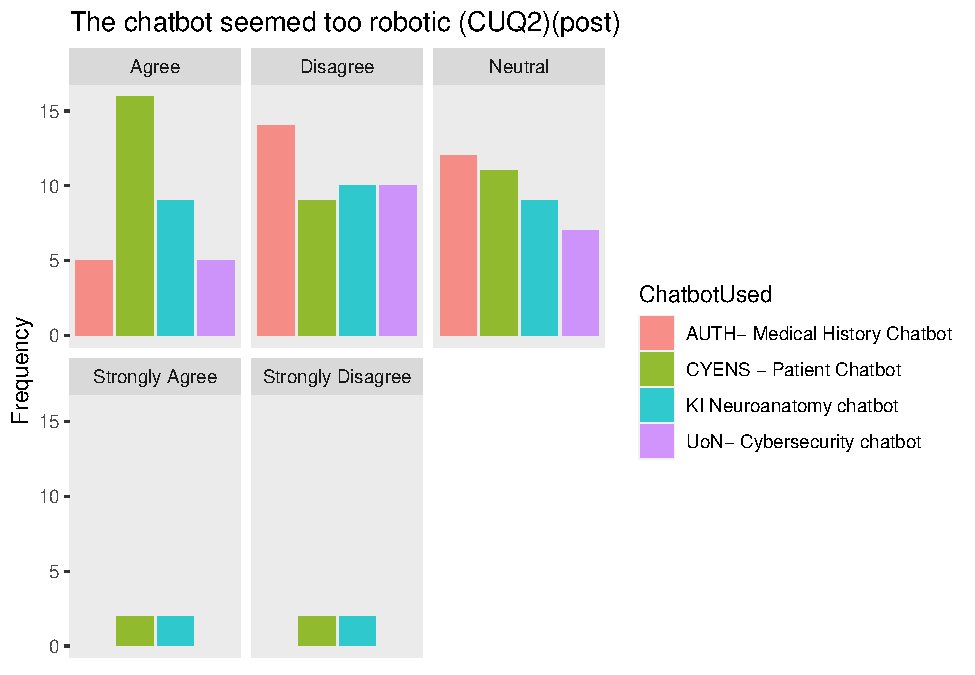
\includegraphics{_main_files/figure-latex/Boxplotsplits8-1.pdf}

\emph{The chatbot seemed too robotic} results had the largest mix of
responses, and for all 4 chatbots evaluated. The University of
Nottingham Cybersecurity chatbot had more deterministic pathways with
exploitation of the NLP modelling to provide illusion of realism. This
may explain why there was less agreement. However, Neutrality and/or
agreement was not desired.

The CYENS medical patient chatbot had more complex pathways of
interactions,

\hypertarget{ease-of-use-and-seeking-support}{%
\subsection{Ease of Use and Seeking Support}\label{ease-of-use-and-seeking-support}}

\begin{figure}
\centering
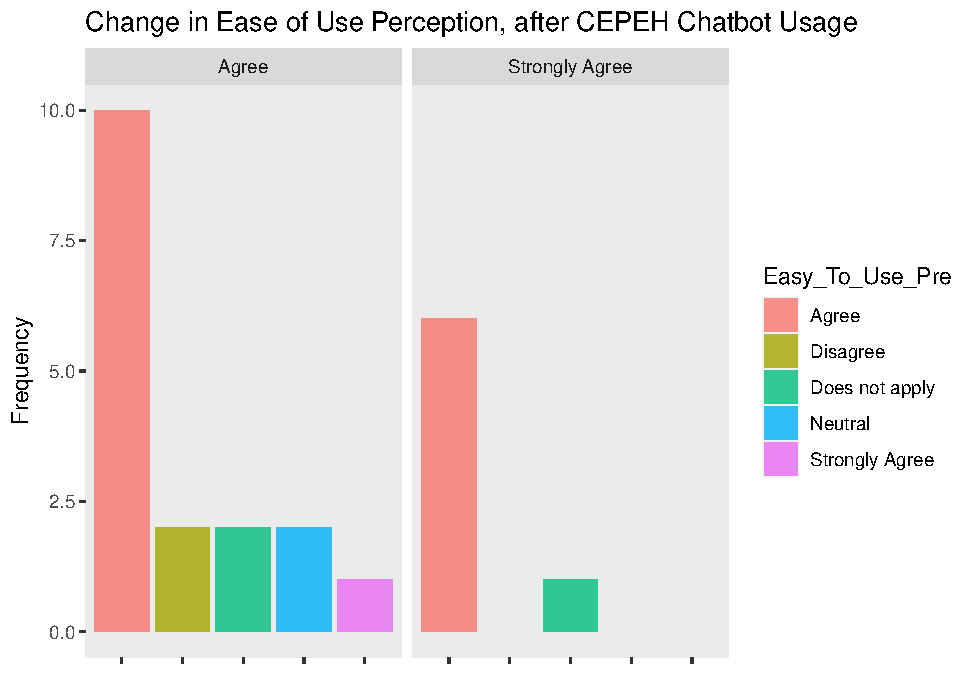
\includegraphics{_main_files/figure-latex/Boxplotsplits9-1.pdf}
\caption{\label{fig:Boxplotsplits9}Ease of Use Comparison}
\end{figure}

After usage, there was only agreement in Ease of Use- as shown in
(\ref{fig:Boxplotsplits9} as there are no `Neutral' or disagree
columns. Any learners with disagreement before using the CEPEH chatbots,
after believed they were easy to use.

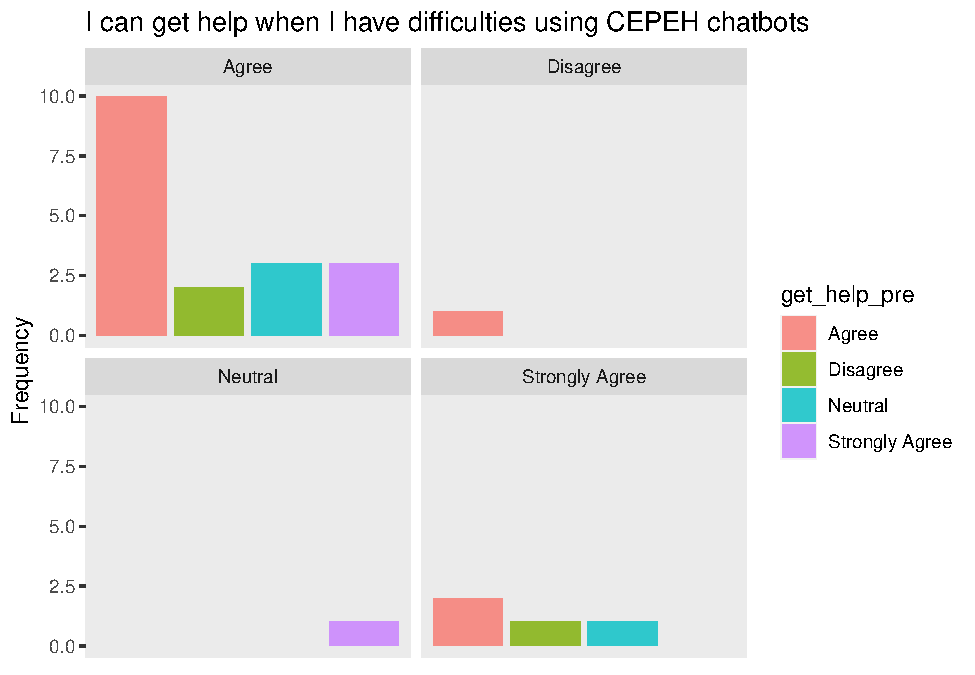
\includegraphics{_main_files/figure-latex/Boxplotsplits10-1.pdf}

Those who disagreed or were neutral in the pre usage measure, improved
their understanding that help was available with the CEPEH chatbots.
After usage, 40 participants agreed they could get help if they had
difficulty using the resources.

\hypertarget{inferential-statistics}{%
\section{Inferential Statistics}\label{inferential-statistics}}

\hypertarget{repeated-measures-t-test-results}{%
\subsection{Repeated Measures T-test results}\label{repeated-measures-t-test-results}}

After using the CEPEH chatbots, majority of participants stated they
would reuse the chatbots. However, there was 6 counts of \emph{disagree} or
\emph{strongly disagree} for all 4 chatbots. Further, there were 17 counts of
neutral in reuse, which was approximately 4 participants per chatbot
(see (\ref{fig:Boxplotsplits4}).

\begin{figure}
\centering
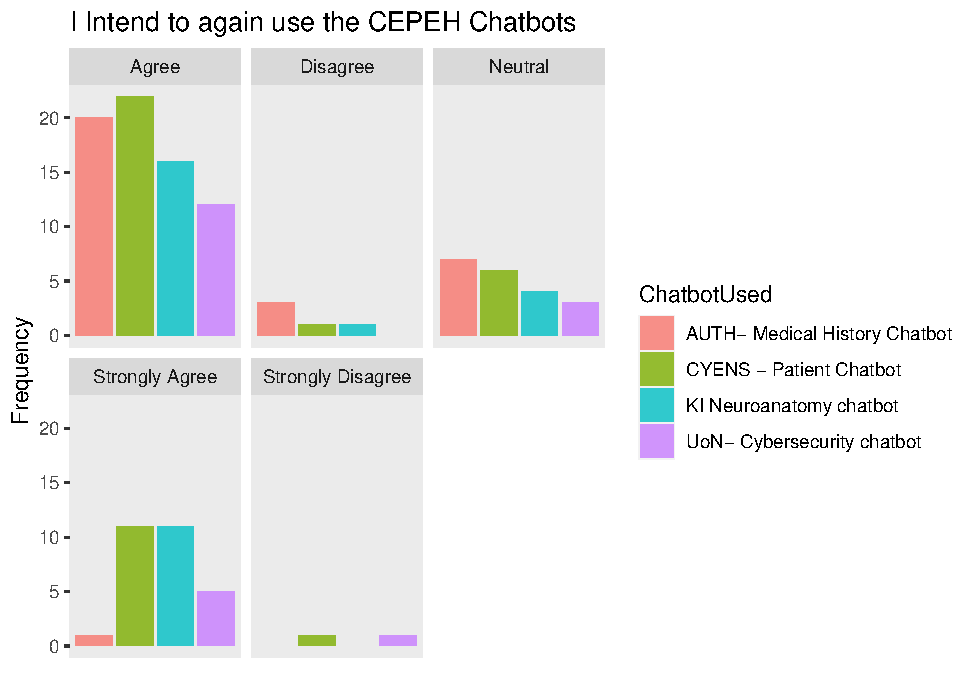
\includegraphics{_main_files/figure-latex/Boxplotsplits4-1.pdf}
\caption{\label{fig:Boxplotsplits4}Intend to Reuse-Post}
\end{figure}

For CYENS, even though the knowledge of the topic was not perceived to
improve by some participants, this box plot shows how 34/42 stated they
would reuse the chatbot developed by CYENS.

\begin{figure}
\centering
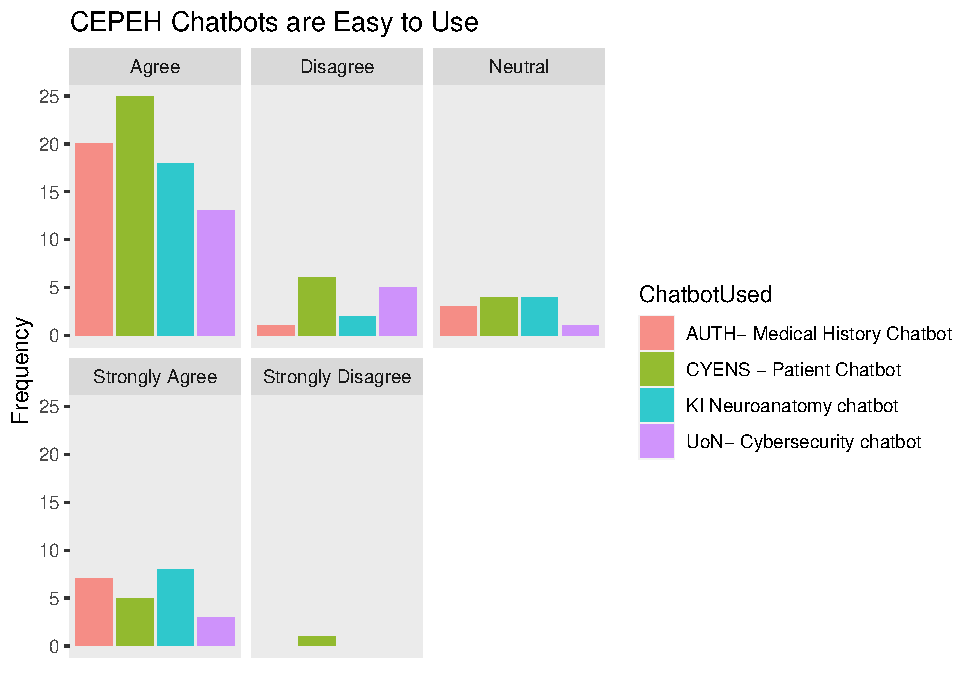
\includegraphics{_main_files/figure-latex/Boxplotsplits3-1.pdf}
\caption{\label{fig:Boxplotsplits3}Easy to Use- Post}
\end{figure}

There was only 1 `Strongly Disagree' response. The agreement options
counted for the majority of the data.

\hypertarget{other-findings}{%
\section{Other Findings}\label{other-findings}}

Other questions

I intend to continue using chatbots in the future (BI1)

The chatbot provided the information I needed with minimal commands

My knowledge of the topic improved after i had used the Chatbot

My confidence in understanding the topic improved after I had used the
Chatbot

The chatbot provided me with the type of response i expected from asking
a tutor/lecturer

The information provided was reliable

The chatbot has a high level of trustworthiness

The duration of conversations to find my answer was too long

The videos/images provided were useful to my questions

The chatbot exceeded my expectation of how it could help me

The chatbot exceeded my expectation of how it could engage with me

I think this learning method could help me to acquire knowledge

I would use this tool again as it has some value to me

I think I will actively use this learning method

I believe I had some choice about learning during chatbot use

I would trust the chatbot to provide me with information for my course

One piece of knowledge I learned from the chatbot was..

Repeated Measures t-test, aka paired t-test (before and after
measurements)

This t-test compares confident using mobile chatbots before and after
CEPEH chatbot usage.

\hypertarget{cepeh-focus-group-discussion-analysis}{%
\chapter{CEPEH Focus Group Discussion Analysis}\label{cepeh-focus-group-discussion-analysis}}

The focus group discussions provided a lot of feedback for how the participants experienced their interactions with the chatbots, and how the CEPEH team can improve them, improve the design and development processes, and improve uptake and sharing.

One method of analysing this data is with use of text mining and data manipulation, creating word clouds, sentiment analysis, and using a model which can distinguish the unique themes in text, and highlights for us what text is used to create these themes.

Therefore, we have created a model to allow efficient and intelligent analysis of this open/free focus group data.

\hypertarget{tokenising}{%
\section{Tokenising}\label{tokenising}}

Firstly, we tokenised the words from the FGDs. A Token is ``a meaningful unit of text, most often a word, that we are interested in using for further analysis''. For each word we give it a property that we can call upon later.

The data manipulation for this included removing punctuation, converting to lower-case, and setting word type to word (and not such types as ``characters'', ``ngrams'', ``sentences'', ``lines'' etc)

\hypertarget{stop-words}{%
\subsection{Stop words}\label{stop-words}}

The model then removed words with meaningless function. These are called stop words. Words like ``the'', ``of'' and ``to'' are the most frequent words found, technically, but are of little interest to us.

We also created a custom list of stop words for CEPEH. We know participants may mention other objects, and the list was as followed: found; chatbot; chatbots; presentation.

The data was ready for analysis by the model. We ordered it to find the most frequent words.

\begin{verbatim}
## # A tibble: 384 x 3
## # Groups:   doc_id [1]
##    doc_id word            n
##    <fct>  <chr>       <int>
##  1 1      information    11
##  2 1      helpful         8
##  3 1      understand      8
##  4 1      idea            7
##  5 1      ideas           7
##  6 1      workshop        7
##  7 1      beginning       6
##  8 1      dont            6
##  9 1      medical         6
## 10 1      technology      6
## # ... with 374 more rows
\end{verbatim}

\hypertarget{plotting-word-frequencies---bar-graphs}{%
\section{Plotting word frequencies - bar graphs}\label{plotting-word-frequencies---bar-graphs}}

With this information a Bar graph of top words from the participants in the FGD can be rendered.

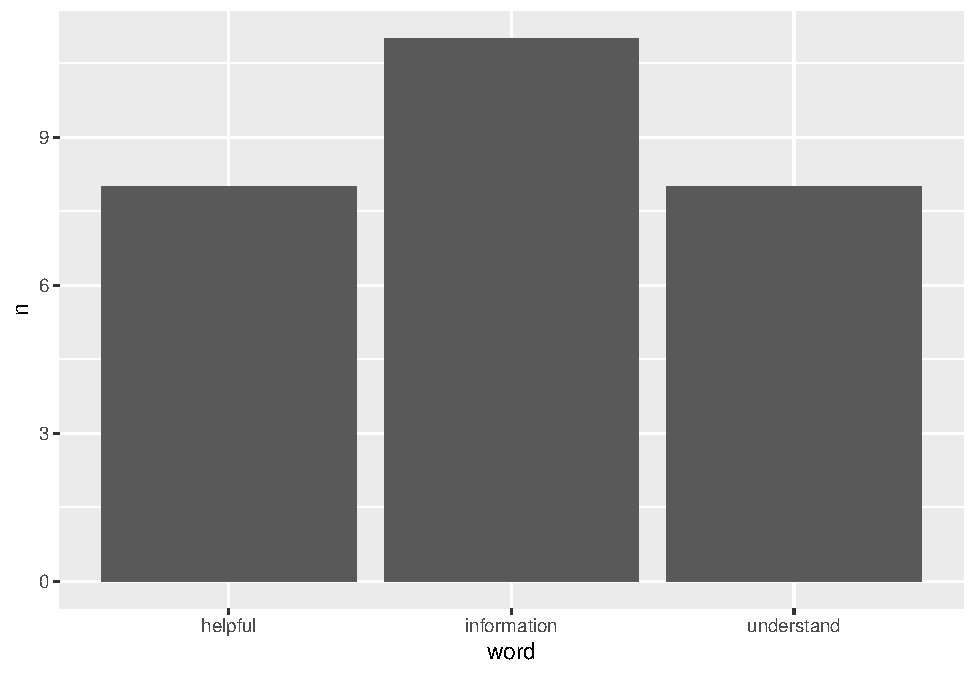
\includegraphics{_main_files/figure-latex/FREQ words bar graph-1.pdf}

and after some modifications, a graph of the top 35 words is produced, with better aesthetics.The most frequent words present in focus group discussions after using the 4 chatbots, are in the Figure below.

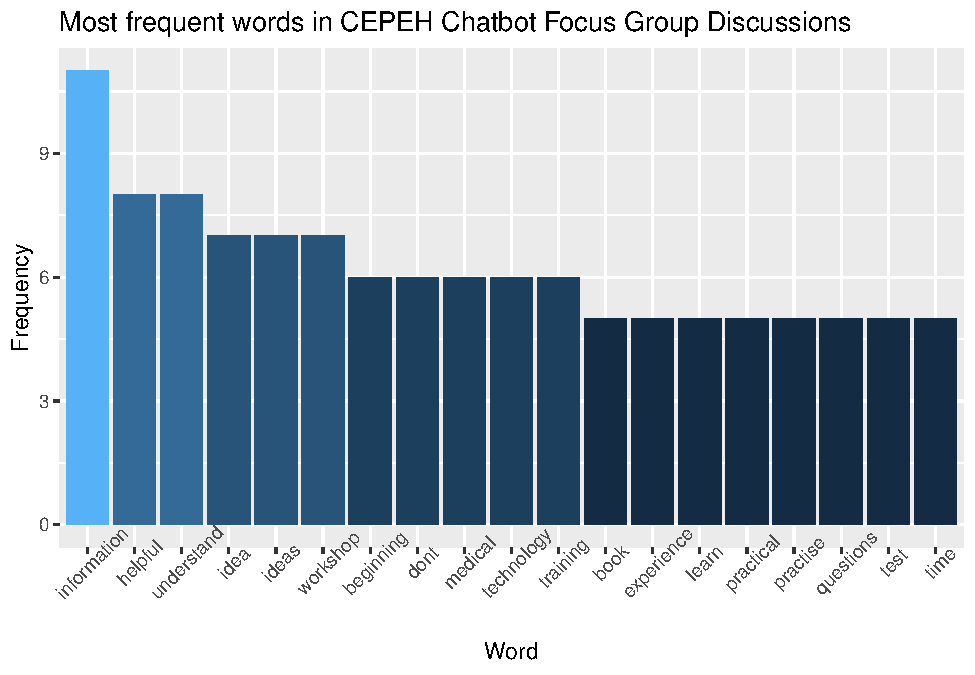
\includegraphics{_main_files/figure-latex/unnamed-chunk-7-1.pdf}

Although the frequency is not high for each word, we are able to get a general picture of the sentiments, intensities, and concerns which would be immediately occurring when plotted.

\hypertarget{normalised-frequency}{%
\subsection{Normalised frequency}\label{normalised-frequency}}

A better way to understand this data is to normalise the frequency of occurrences in accordance with the source text. The raw text had 2827 words in total. Therefore we can mutate the ratios to reflect this.

\hypertarget{plotting-normalised-frequency}{%
\subsection{Plotting normalised frequency}\label{plotting-normalised-frequency}}

Now we can plot, for example, the 20 most frequent words when normalised by the source text.

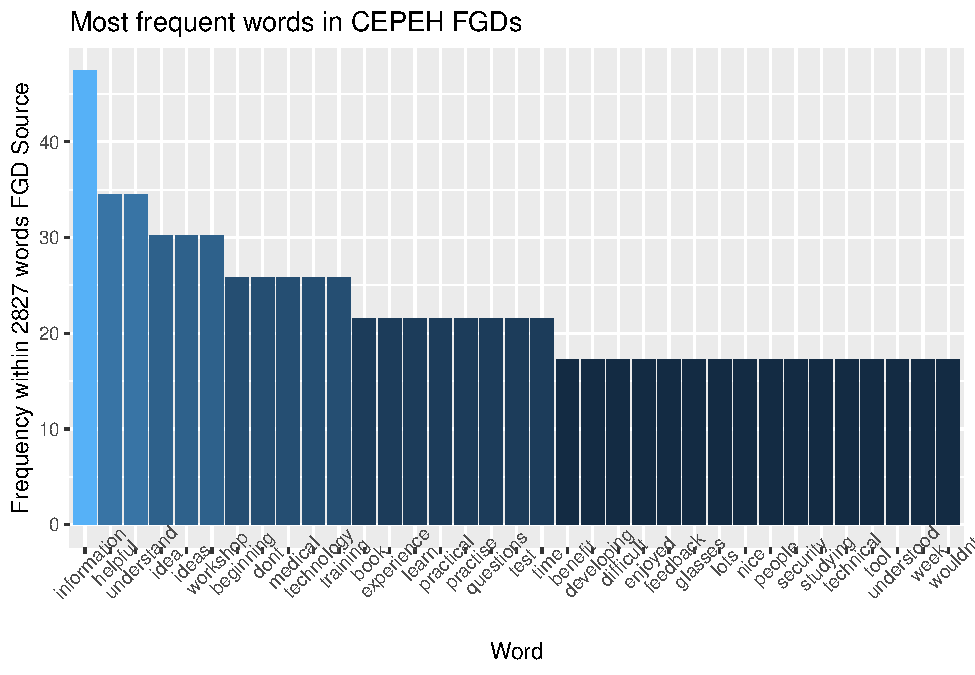
\includegraphics{_main_files/figure-latex/CEPEH MOST FREQ-1.pdf}
In summary, this understanding of frequent words can help to understand common concurrences and extrapolate to a larger audience. If scope and impact of CEPEH chatbots increased we can understand the type of themes and trends may occur, based on such FGD analysis.

\hypertarget{word-clouds}{%
\section{Word clouds}\label{word-clouds}}

To visualise the most frequent words in another format, below is a word cloud which presents the word size to indicate the frequency- words that occur more often being displayed in a larger font size.
This has a normalised data frequency in accordance to the FGD source document analysed.

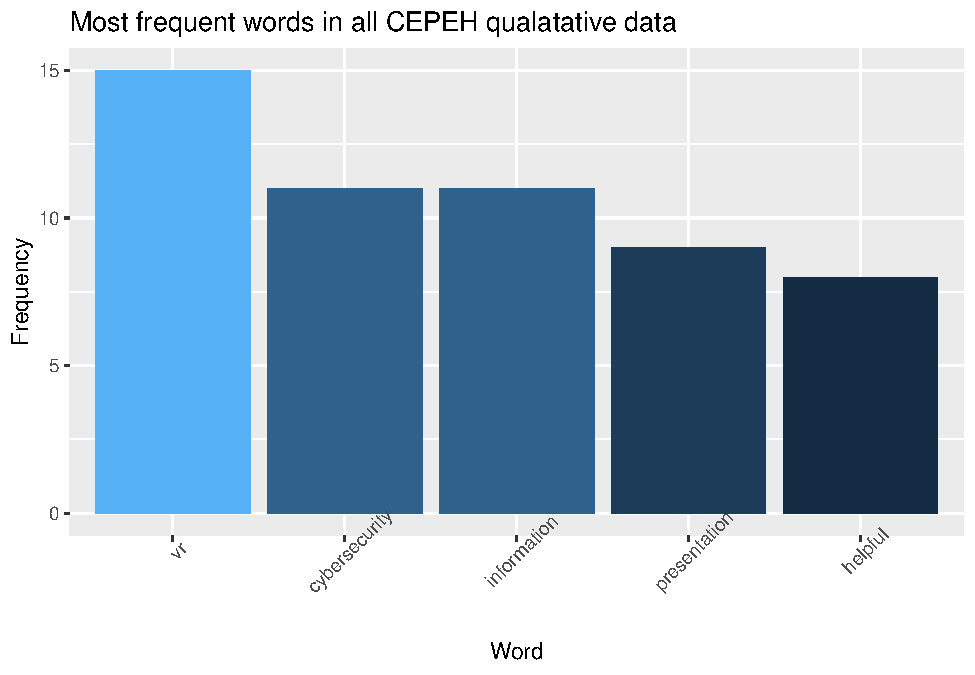
\includegraphics{_main_files/figure-latex/unnamed-chunk-9-1.pdf}
We understand the context has been reduced for each word. However, in general there can be categorised positive/negative words from the word cloud:
Positive words are- benefit, practical, nice, helpful, learn, ideas, and enjoyed
Negative words are- difficult, test (who likes a test?), don't, and `lot' may be negative if there is a `lot' of information.

\hypertarget{the-vocabulary-of-texts}{%
\subsection{The vocabulary of Texts}\label{the-vocabulary-of-texts}}

Here is a graph that has plotted the words in places depending on the word frequencies. Additionally, colour hotspots shows how different the frequencies are - darker items are more similar in terms of their frequencies, lighter-coloured ones more frequent in one text compared to the other.

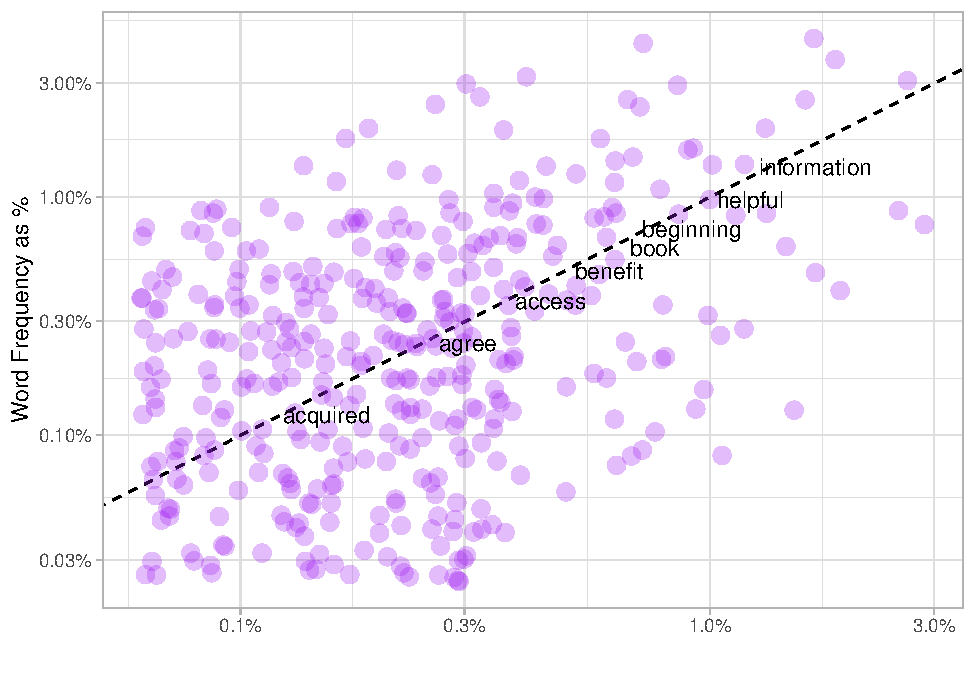
\includegraphics{_main_files/figure-latex/unnamed-chunk-11-1.pdf}

\hypertarget{sentiment-analysis}{%
\section{Sentiment analysis}\label{sentiment-analysis}}

What is the sentiment of all participants? What is types of emotional words are being used?
The preparation of these words has some use in understanding the frequencies, but their emotional valence are not compared. The table above has the word \emph{`helpful'} which has a positive connotation, however there are 386 words, with many having several occurrences.

\begin{verbatim}
##   max(total_score) min(total_score)
## 1               38               38
\end{verbatim}

\begin{tabular}{r|r|r}
\hline
negative & positive & total\_score\\
\hline
24 & 62 & 38\\
\hline
\end{tabular}

\hypertarget{Discussion}{%
\chapter{Discussion}\label{Discussion}}

\minitoc 

\#\#Summary of Findings

The Chatbots were beneficial.

Learners have lots of other choices such as YouTube, but there is a certain need for personalised information gathering , this can save time and prevent learning incorrect information.

This was one reason why they were rated positive as they are able to streamline data finding for learners in a format that is understandable and easy to them.

\hypertarget{quantatative-results}{%
\section{Quantatative Results}\label{quantatative-results}}

\hypertarget{cuq}{%
\subsection{CUQ}\label{cuq}}

Holmes et al.~{[}\url{https://dl.acm.org/doi/10.1145/3335082.3335094}{]} designed the CUQ to be comparable with the system usability scale (SUS).

We have calculated both these scores out of 100 to allow the same benchmark, which is 68. A score of 68 is at the centre of the range is thought of as ``C''. The average benchmark for CUQ is 68, and in initial/pilot studies 68 may be considered higher than expected when considering technical issues, less developed user interfaces etc.

Previous studies evaluating chatbots have had similar score. For
example, in 2022 \href{a\%3C\%20href=}{Link} found a
physical activity promotion chatbot received 64.5/100, with lowest score
at 40.6

\hypertarget{qualatative-results}{%
\section{Qualatative Results}\label{qualatative-results}}

\hypertarget{limitations}{%
\section{Limitations}\label{limitations}}

\hypertarget{conclusions}{%
\section{Conclusions}\label{conclusions}}

Those results can be interpreted that the learning objectives of the training event was chosen appropriately for the diverse audience including clinicians, academics, researchers, and learning technologists/IT specialist resulting to a successful training event that enable participants to take the acquired knowledge back to their organisations in order to co-design and implement. As it was expected and can be depicted from self-confidence statements that some participants being very confident before the event, not all the objectives expected to be reached by everyone, since the training was targeting both technical and non-technical participants. However, on both average and individual matched responses participants self-statements showed that they improved their knowledge and understanding in using co-creation approaches to develop digital education resources and in designing and developing chatbots as educational resources.

output:
\#bookdown::html\_document2: default
\#bookdown::word\_document2: default
bookdown::pdf\_document2:
template: templates/template.tex
documentclass: book

\hypertarget{cites-and-refs}{%
\chapter{(Additional Analyses) Training Events}\label{cites-and-refs}}

\chaptermark{Citations and cross-refs}

\minitoc 

\hypertarget{cepeh-training-event-c1}{%
\section{CEPEH Training Event C1}\label{cepeh-training-event-c1}}

The CEPEH training event C1 held at the premises of University of Nottingham aiming to prepare participants for the practical elements of co-creation and implementation of chatbots as an educational resource. It combined both theoretical and hands-on training.
15 participants were from RISE, AUTH, UoN.

Project managers of partners signposted the person involved, and relevant announcements were made though social media channels to the wider public. External to the project speakers were from University of Leeds, and Computer Science Department of University of Nottingham. It included academics, medical doctors, and researchers with focus both on clinical research and digital innovations in healthcare education and IT specialist/learning technologists 11.18 years of experiences (SD=7.2). A balance between male and female participants achieved.

Participants were asked to highlight what they liked for each day and how each day can be improved. Findings are described below per day of the training event

Day 1\\
The participants comment that they liked the design method for educational resources presented using a co-creation approach, they liked the interactions with other groups, and they liked the overview of existing chatbot resources of the partners. On the areas that can be improved, more media material were requested.

Day 2
Participants enjoyed the presentation from the invited speaker from another faculty of the University of Nottingham, the CEPEH recources presented and the storyboarding process. Participants highlighted that the participation of more clinicians in the event would be an added value in regards with the storyboarding process.

Day3
Participants liked the hands-on activities of the day also enjoyed the creativity of the groups on the online chatbot development tool. As an area of improvement, participants wanted more time on hands on sections.

\hypertarget{cepeh-training-event-2}{%
\section{CEPEH Training Event 2}\label{cepeh-training-event-2}}

\textbf{Pre-Training Event survey May 9th-13th 2022 Thessaloniki, Greece}

Twenty-six participants attended the Training Event, along with approximately 10 staff members. There were 21 undergraduate students and 5 postgraduate students, who completed the survey for a total of 26 responses. There were 86\% of participants who stated they had not been to a similar event like the training event CEPEH facilitated. There were 90\% of students who found the event schedule very organised, and 70\% agreed most of the planned sessions were relevant to that interest with the remaining 30\% not having enough experience to understand the context to determine if they are interested in the training event. There were 95\% of students agreeing or strongly agreeing the training event location is great, the remaining person did not leave additional comments.

Table 1 suggested attendees had minimal intention to share their own ideas due to lack of previous experience of attending such events, or due to lack of knowledge on the area. However, most were interested in listening to other groups and hearing contextual cases in healthcare.

There were 77\% of participants stated they were novices in experience with chatbots in healthcare and were attending to learn more. The remaining 23\% (7 students) stated they were competent and had limited experience with chatbots in healthcare.

One day had several events regarding cybersecurity in healthcare. When asked before these events, 83\% stated they were neutral or disagreed that they felt confident about their cybersecurity knowledge in healthcare. In addition, 80\% stated they when neutral or disagreed that they felt they had strong cybersecurity safety in healthcare. Table 2 shows the main pre and post results suggesting a positive experience for more than 75\% of attendees on all measures.

There were 90\% (23) of students who heard about the event through a lecturer or a professor, the CEPEH newsletter (2), and 1 person was informed through the anatomy tutoring system at Karolinska Institute. Additionally, 60\% suggested the training event to somebody else before the course started.

There were six individuals who stated neutral or disagree when asked if having issues on registration or finding the information for the event. This may have been due to being dependent on emails to receive the information, instead of a dedicated website where the information is available anytime.

As this was face-to-face, participants were asked about sufficient Covid-19 precautions in place at the facility, 94\% agreed with sufficient precautions, two individuals stated no but did not give further information in the additional input box provided.
In summary, most participants were undergraduate students with novice experience, happy with the training event location, felt the sessions were relevant to them, and most shared the event with their colleagues. The values of co-creation, chatbots in healthcare, and taking patient history were bestowed to students in an engaging and well-received manner. Notably, the highest ratings were for staff friendliness which is key to engagement and consistent interaction throughout the intense and long 5-day duration. The sessions were recorded there for the online recordings may be viewed with higher numbers over the subsequent weeks.

\hypertarget{bibliography-bibliographyreferences.bib-bibliographyadditional-references.bib}{%
\section{\# bibliography: {[}bibliography/references.bib, bibliography/additional-references.bib{]}}\label{bibliography-bibliographyreferences.bib-bibliographyadditional-references.bib}}





\hypertarget{appendix}{%
\chapter*{Appendix}\label{appendix}}
\addcontentsline{toc}{chapter}{Appendix}

\startappendices

\hypertarget{the-first-appendix}{%
\chapter{The First Appendix}\label{the-first-appendix}}

This first appendix includes an R chunk that was hidden in the document (using \texttt{echo\ =\ FALSE}) to help with readability:

\textbf{In 02-rmd-basics-code.Rmd}

\textbf{And here's another one from the same chapter, i.e.~Chapter \ref{code}:}

\hypertarget{references}{%
\chapter*{References}\label{references}}
\addcontentsline{toc}{chapter}{References}

\markboth{References}{}

\hypertarget{refs}{}
\begin{CSLReferences}{1}{0}
\leavevmode\vadjust pre{\hypertarget{ref-Darwin1859}{}}%
Darwin, C. (1859). \emph{{On the Origin of Species by Means of Natural Selection or the Preservation of Favoured Races in the Struggle for Life}}. John Murray.

\leavevmode\vadjust pre{\hypertarget{ref-von_goethe_wilhelm_1829}{}}%
Goethe, J. W. von. (1829). \emph{Wilhelm {Meisters} {Wanderjahre} oder die {Entsagenden}}. Cotta.

\end{CSLReferences}

%%%%% REFERENCES


\end{document}
